\documentclass[12pt, letter]{article}

% Load packages
\usepackage[style = authoryear, autocite=inline, doi=false,isbn=false,url=false]{biblatex}
\usepackage[margin = 1 in]{geometry}
\usepackage[colorlinks, citecolor = red]{hyperref}
\usepackage{amsmath, amssymb} %essential
\usepackage[long, nodayofweek]{datetime}
\usepackage[]{booktabs}
\usepackage{graphicx}
\usepackage{setspace}
\usepackage{todonotes}
\usepackage[font=small,labelfont=bf]{caption}

% Define symbols
\DeclareRobustCommand{\bbone}{\text{\usefont{U}{bbold}{m}{n}1}}
\DeclareMathOperator{\EX}{\mathbb{E}} % expected value
\DeclareMathOperator{\V}{\mathbb{V}}
\DeclareMathOperator{\Prob}{\mathbb{P}}
\newcommand*{\trans}{^{\mathsf{T}}} %matrix transpose


\begin{document}

% Define Header
\author{Andrew C. Eggers\thanks{Nuffield College and Department of Politics and International Relations, University of Oxford, United Kingdom. \texttt{aeggers@nuffield.ox.ac.uk}}
\and
Tobias Nowacki\thanks{Department of Political Science, Stanford University, CA, United States. \texttt{tnowacki@stanford.edu}}}
\date{\today}
\title{Comparing strategic voting incentives in plurality and instant-runoff elections}

\maketitle

\onehalfspacing % set line space

\setcounter{section}{4}

\section{Data}

To assess the prevalence and distribution of strategic incentives under Plurality and IRV empirically, we rely on data from the  Comparative Study of Electoral Systems (CSES) for a realistic set of preferences and beliefs. The dataset covers 160 surveys from xx different countries, administered shortly before or after an election.\footnote{Two additional cases in the survey, Belarus (20xx) and Lithuania (20xx), are dropped because no respondent specified full preferences over more than two parties.} We focus on the three largest parties (evaluated how?) and label them $A, B, C$ in descending size, respectively. From each survey in the data set, we take respondents' party like/dislike scores for these parties to approximate voters' ordinal utilities and, by extension, their preferences over the parties.

Let $\bf \tilde{v}$ be the vector of ballot proportions if everyone in the CSES survey voted sincerely according to their preferences. If voter $i$ believes that everyone else is voting sincerely (in other words, everyone else is Level-0 strategic), then we model the $i$'s belief about the next election as $\text{Dir}(s \times \bf \tilde{v})$, where $s$ is a parameter capturing the precision of $i$'s beliefs. Given this set-up of beliefs and preferences, we calculate the strategic incentives under either electoral system, and iterate this procedure as laid out in Section 3.

The remainder of this section describes brief summary statistics of the CSES data.


\subsection{Summary statistics}

\begin{figure}[!htb]
	\centering
	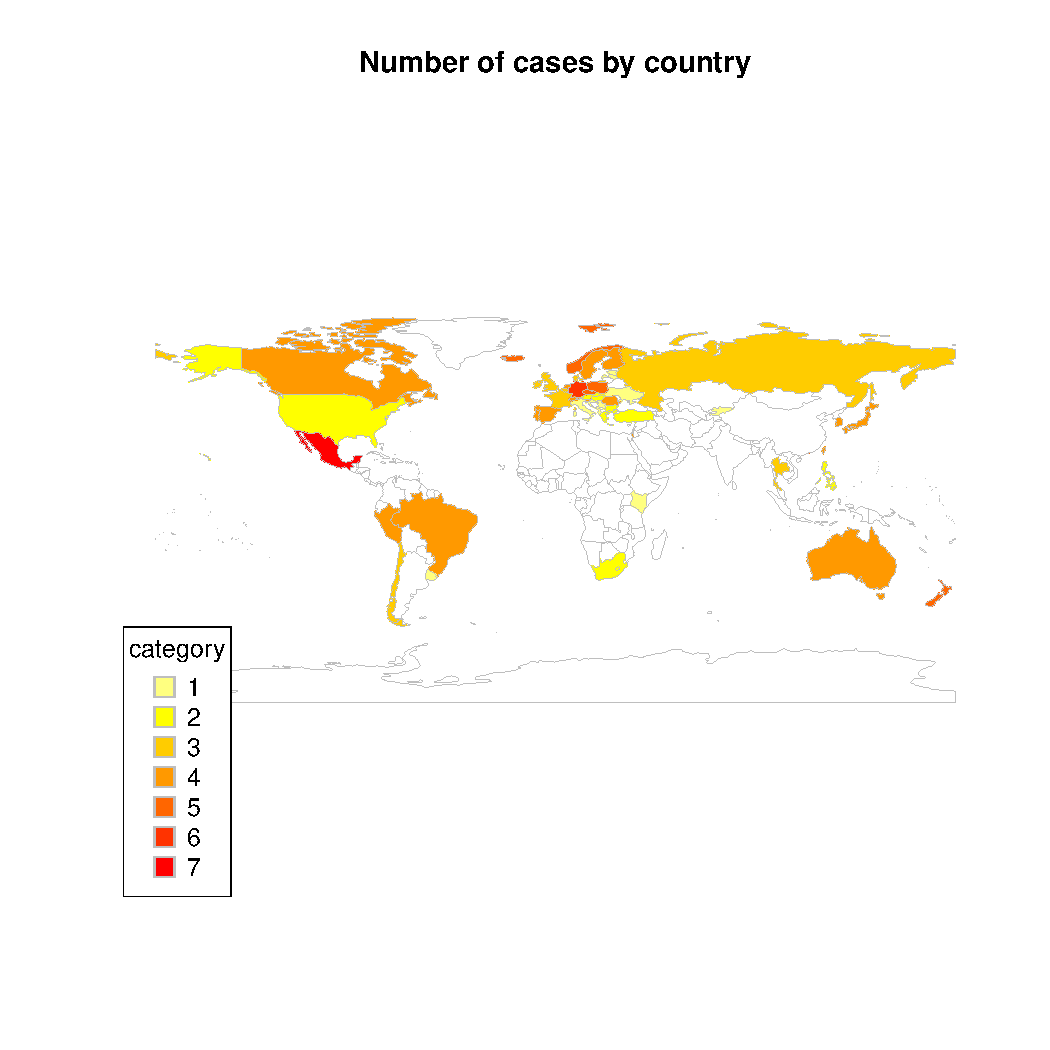
\includegraphics[width = .5 \textwidth]{../output/figures/case_map.pdf}
	\caption{Cases in CSES data, by country}
	\label{fig:case_map}
\end{figure}

The mean number of respondents in the CSES surveys is 1384 (with a standard deviation of 539). The 160 different surveys come from xx different countries, between 1996 and 2016. Figure~\ref{fig:map} maps the number of surveys in each country. (Do we need to say any more? Perhaps something about mean / sd of preference intensity and $\tau$?)

\subsection{Weighting}

In some CSES cases, respondents are assigned a non-uniform weight. When computing case-level statistics (e.g., prevalence of strategic incentives in case $j$), we weigh each observation by its original weight. When aggregating up even further, and presenting aggregate statistics (averaged over all cases), we also assign case-level weights to adjust for countries' voting age population and the overrepresenation of some countries.\footnote{Recall that our initial objective is to compare the \textit{overall} distribution of strategic voting incentives under Plurality and IRV. Without weights, we would run the risk of having our findings distorted by a small countryoutlier that counts for as much as a large state (e.g., Denmark and the United States); alternatively, we also do not want a result that is particular to one country to be over-represented purely because there are multiple surveys from that country.}

These case-level weights are constructed as follows:

\begin{equation}
	w_j \equiv
\end{equation}

\subsection{Distribution of preferences} 

How different are the CSES cases from one another? Aside from the intensity of preferences, we can describe each case with the vector $\bf \tilde{v}$, where the three-item vector $(v_1 + v_2, v_3 + v_4, v_5 + v_6)$ describes the distribution of first preferences, and the three-item vector $(m_{AB} = \frac{v_1}{v_1 + v_2}, m_{BA} = \frac{v_3}{v_3 + v_4}, m_{CB} = \frac{v_6}{v_5 + v_6})$ describes the distribution of second preferences. 

To link these two distributions together and classify cases more completely, we offer the following approach. Without loss of generality, let the candidate (party) $X$ whose first-preference voters have the most equally split second preferences, and the other two parties $Y$ and $Z$. If both $m_{YZ}$, $m_{ZY} > 0.6$, then classify this case as \emph{single-peaked} and denote it $X+$.\footnote{$X$ is the attractor: both remaining parties have a majority of their second preferences tilted towards $X$.} Conversely, if both $m_{YZ}, m{ZY} < 0.4$, then classify this case as \emph{divided majority} and denote it $X-$.\footnote{Here, $X$ is the repeller: both remaining parties have a majority of their second preferences tilted towards each other and away from $X$.} If $m_{YZ}, m_{ZY} \in [0.4, 0.6]$, then classify this case as \emph{neutral} and denote it $N(X)$. If neither of these conditions hold (because of unusual second preferences), classify it as \emph{other} and denote it $O$. This completes a mutually exclusive and exhaustive set of classes determined by $\bf \tilde{v}$.

\begin{table}[tb]
	\caption{Distribution of preference profiles in CSES data}
	\label{tab:csesprefs}
	\centering

	\begin{tabular}{lccc}
	\hline

	\toprule
	\textbf{} & \textbf{A} & \textbf{B} & \textbf{C} \\
	\cmidrule{2-4}
	Single-peaked (+) & 18 & 23 & 9  \\
	Divided majority (-) & 28 & 20 & 20  \\
	Neutral () & 5 & 7 & 3  \\
	Other () & & 27 &  \\
	\bottomrule
	\end{tabular}
\end{table}

Table~\ref{tab:csesprefs} summarises the distribution of preference classes across the CSES cases. A plurality of cases belong to the divided majority classes; however, there is also a large number of single-peaked cases, whereas neutral and others tend to be rarer. (Figure~\ref{fig:cses_fp} plots the distribution of first preferences conditional on the classes.)

\begin{figure}[!htb]
	\centering
	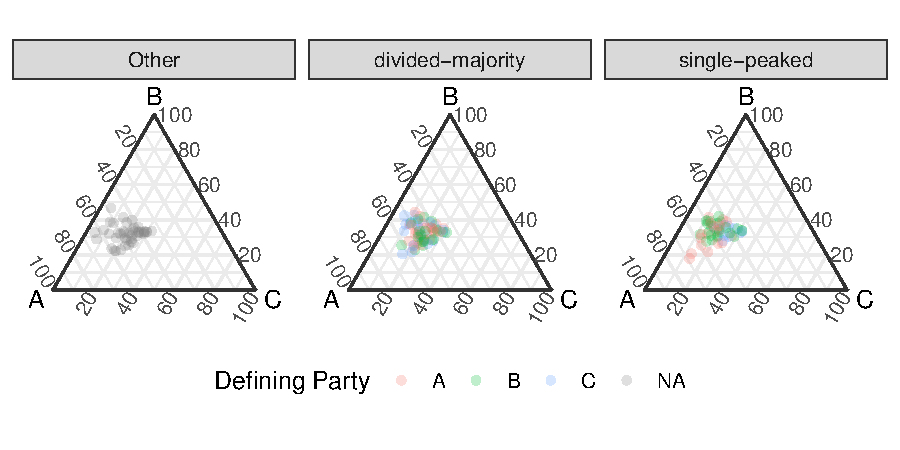
\includegraphics[width = 0.6 \textwidth]{../output/figures/cses_fp.pdf}
	\caption{Distribution of first preferences in CSES cases, by class}
	\label{fig:cses_fp}
\end{figure}

\section{Results}

We now proceed to present and discuss our results.

\subsection{Convergence}

Under both IRV and Plurality, the distribution of ballot shares quickly converges towards a fixed point in the vast majority of CSES cases. The average Euclidean distance going from the 59th to the 60th iteration is below 0.0014 for Plurality, and below 0.006 for IRV.\footnote{These averages are unweighted -- need to recompile in the future.} Put differently, we can obtain a perfectly strategic voting equilibrium, where all voters anticipate others' vote choices, and react accordingly, within about 60 iterations from the sincere voting profile.

\begin{figure}[!tbh]
	\centering
	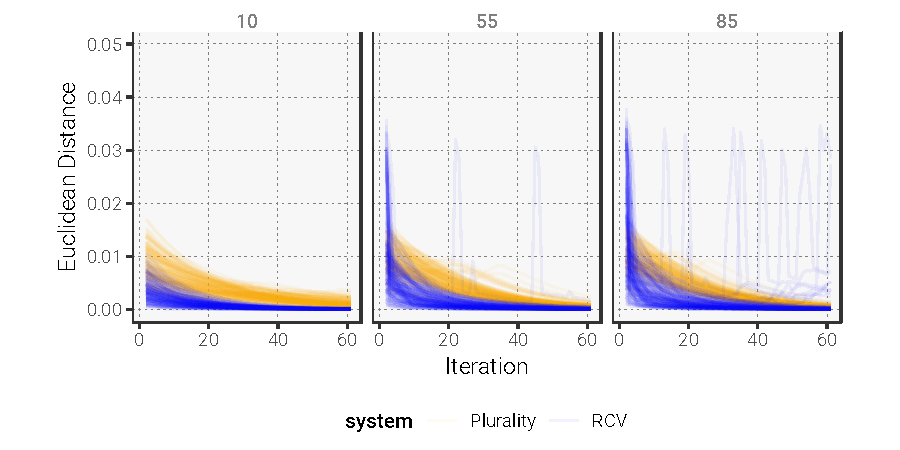
\includegraphics[width = \textwidth]{../output/figures/euclidean}
	\caption{Euclidean distance between ballot share vectors from one iteration to another.}
	\label{fig:convergence}
\end{figure}

Figure~\ref{fig:convergence} plots the Euclidean distance between the ballot shares for every case and iteration under both Plurality and IRV. In expectation, convergence towards the fixed point occurs faster under IRV than it does under Plurality. As we discussed earlier, strategic incentives under Plurality are characterised by complementarity; this means that with every additional iteration, the incentive for supporters of the third party increases, until all of them have deserted the trailing candidate and the ballot shares are in a Duvergian (two-party) equilibrium.\footnote{We could visualise this by plotting the share of third-party votes when $k = 60$.} In contrast, the substitutability of strategic voting incentives under RCV allows them to reach a fixed point much sooner. Note however, that, for more precise beliefs ($s \in {55, 85}$), the shift away from the sincere ballot profile in the first few iterations is much bigger than under Plurality; quicker convergence does not necessarily mean that the fixed point is closer to the original ballot share vector.\footnote{This foreshadows a later result: with sufficiently high precision, the prevalence of strategic voting incentives under IRV will be higher in the first few incentives.}

In sum, when applying our iterative strategic voting procedure to all CSES cases, the ballot shares converge more quickly to a fixed point under IRV than under Plurality. Under IRV, these fixed points can occur anywhere in the ballot share space, whereas under Plurality, voters ultimately settle on a two-party Duvergian equilibrium. This is also illustrated by Figure~\ref{fig:convergence_paths}, which maps the ballot share vectors before the first and the 60th iteration for $s = 85$.

(Figure about distance from sincere profile? -- shows nicely that Plurality fixed points are further away from initial ballot shares.)

\begin{figure}[]
	\centering
	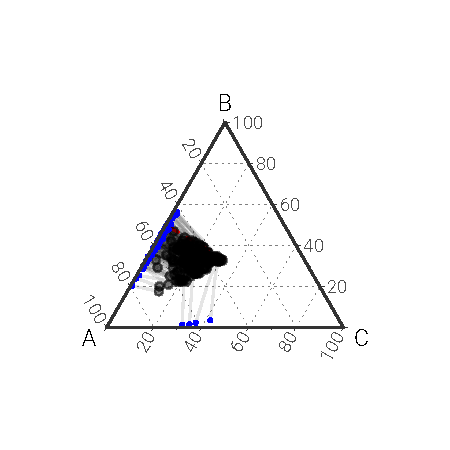
\includegraphics[width = .49\textwidth]{../output/figures/tatonnement_plur}
	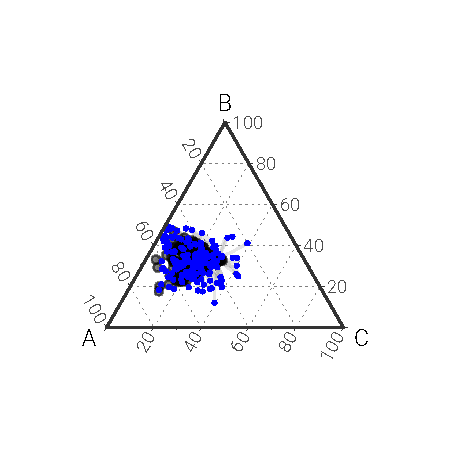
\includegraphics[width = .49\textwidth]{../output/figures/tatonnement_rcv}
	\caption{Evolution of ballot share vectors for all CSES cases over iterations, for both Plurality (left) and IRV (right), when $s = 85$. Grey dots indicate the initial ballot share vector before the first iteration; blue dots the ballot share vector after the 60th iteration.}
	\label{fig:convergence_paths}
\end{figure}

\subsection{Strategic Incentives}

In this section, we present our main results. We focus on the prevalence, magnitude and expected benefit of strategic voting under either electoral system. Overall, strategic voting incentives are more prevalent, have a higher magnitude and higher expected benefit under Plurality than under IRV.

Figure~\ref{fig:main_stats} shows the quantities of interest for each case, as well as the weighted average.

\begin{figure}[]
	\centering
	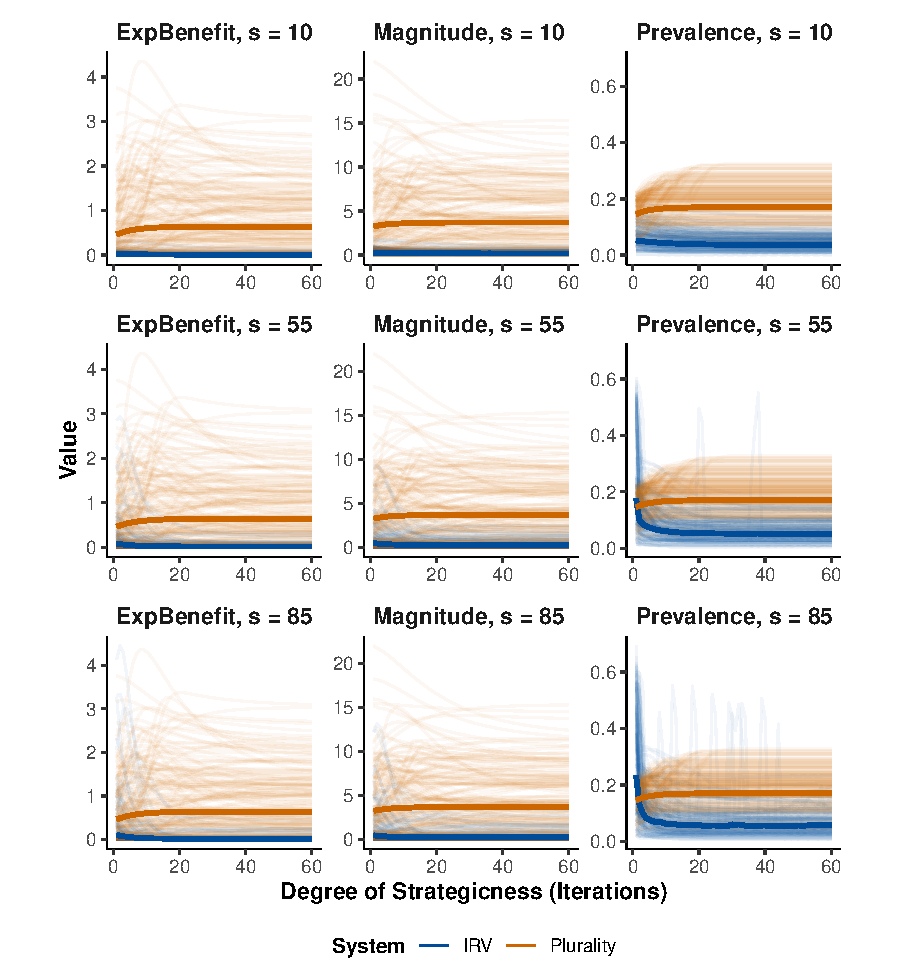
\includegraphics[width = \textwidth]{../output/figures/iterated_complete}
	\caption{Main statistics}
	\label{fig:main_stats}
\end{figure}

\section{Conclusion}



\end{document}